% tags: arc edgeLabel label blockDiagram house background align
\PassOptionsToPackage{usenames,dvipsnames}{xcolor}
\documentclass[tikz, border=10pt]{standalone}

\usepackage{verbatim}
\usepackage{amsmath}

\tikzset{>=stealth}
\tikzstyle{every node}=[align=center]
\usetikzlibrary{spy,shadows,arrows,shapes,positioning,calc,backgrounds,fit,automata}

\newcommand{\Green}{OliveGreen!40}
\newcommand{\Yellow}{GreenYellow!70}
\newcommand{\Orange}{Orange!60}
\newcommand{\Brown}{Sepia!40}
\newcommand{\DarkGreen}{OliveGreen!60}
\newcommand{\DarkOrange}{Orange}
\newcommand{\DarkYellow}{GreenYellow!120}
\newcommand{\DarkBrown}{Sepia!60}
\newcommand{\Blue}{RoyalBlue!30}
\begin{document}
\pgfdeclarelayer{bg}
\pgfdeclarelayer{fg}
\pgfsetlayers{bg,main,fg}
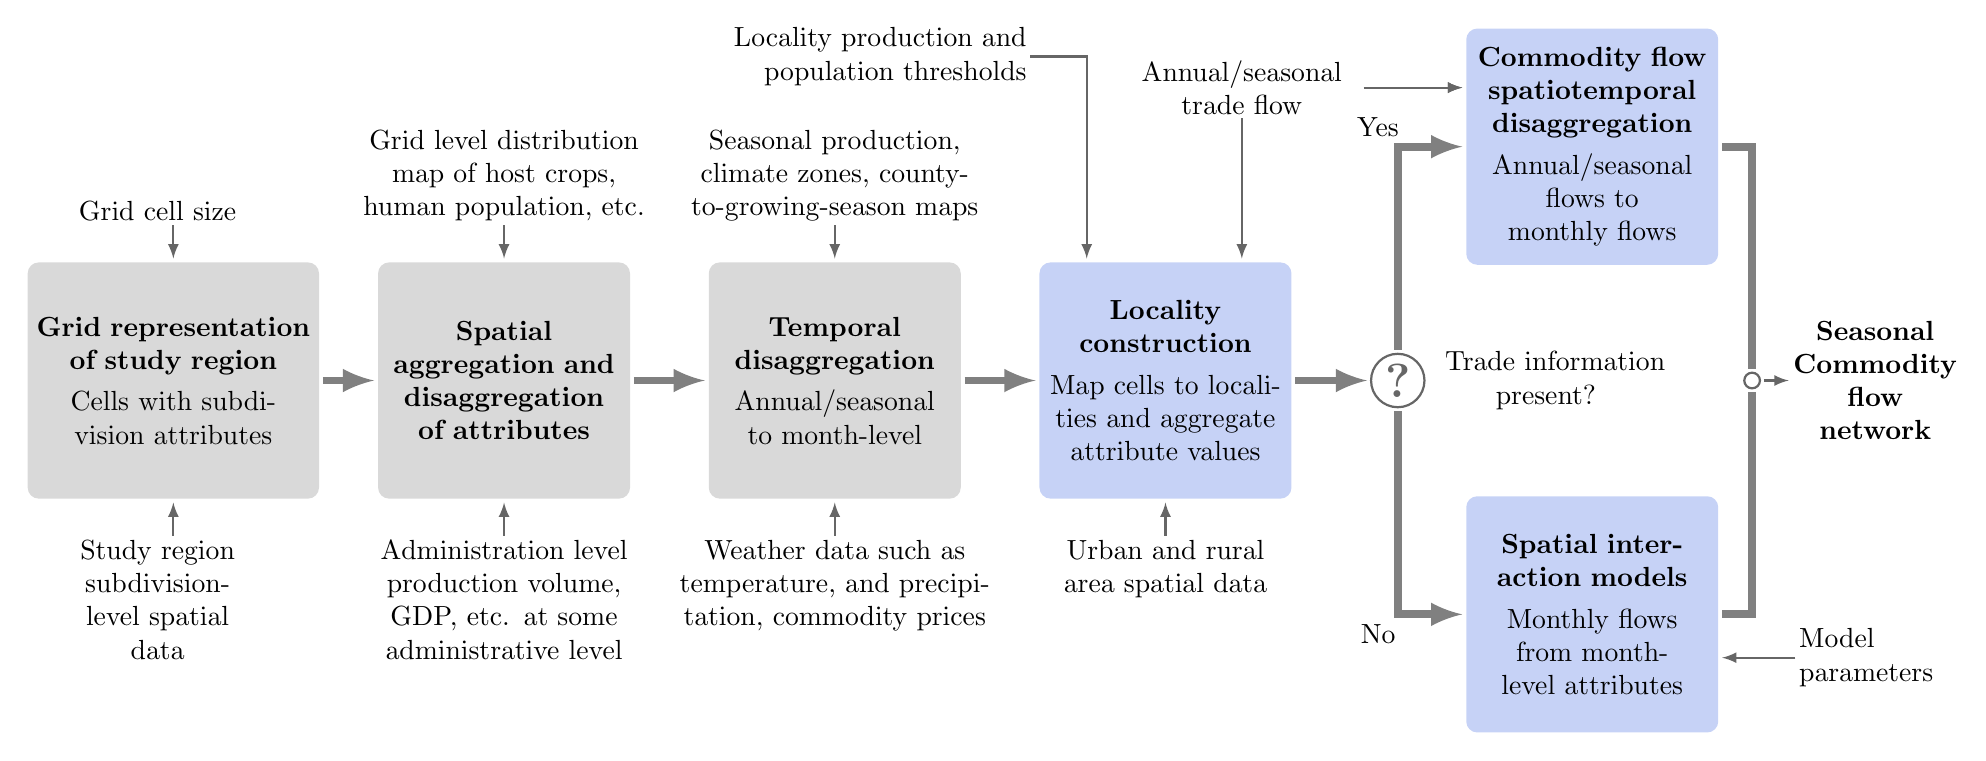
\begin{tikzpicture}
    [font=\normalsize,
        blk/.style={inner sep=.1cm,fill=\Blue,rounded corners,text width=3cm,minimum height=3cm},
every node/.style={inner sep=0,align=center},
blkedge/.style={draw=black!50,>=latex, shorten >=1pt, shorten <=1pt, line
width=1mm},
datedge/.style={draw,>=latex, draw=black!60, shorten >=1pt, shorten <=1pt},
node distance=4.2cm,thick]

%% grid
\node[blk,fill=black!15,text width=3.5cm] (grid) {\textbf{Grid
representation of study region}\\\smallskip Cells with subdivision
attributes};
\node[below of=grid] {};
\draw[datedge,<-] ($(grid.south) + (0,0)$) -- +(0,-.5)
node[shift={(-.2,0)},inner sep=0,text
width=2cm,anchor=north,align=center]{Study region subdivision-level spatial
data};
\draw[datedge,<-] ($(grid.north) + (0,0)$) -- +(0,.5) node[shift={(-.2,0)},inner
sep=0,text width=2cm,anchor=south,align=center]{Grid cell size};
%% spatial
\node[blk,fill=black!15,right of=grid] (spatial) {\textbf{Spatial
        \\ aggregation and disaggregation of
attributes}};
\draw[blkedge,->] (grid) -- (spatial);
\draw[datedge,<-] ($(spatial.south)+(-.0,0)$) -- +(-0cm,-.5cm) node[text
width=4cm,anchor=north] {Administration level production volume, GDP,
etc. at some administrative level};
\draw[datedge,<-] ($(spatial.north)+(+.0,0)$) -- +(0cm,.5cm) node[text
width=4cm,anchor=south] {Grid level distribution map of host crops, human
population, etc.};
%% temporal
\node[blk,fill=black!15,right of=spatial] (temporal) {\textbf{Temporal
    disaggregation} \\
\smallskip Annual/seasonal to month-level};
\draw[blkedge,->] (spatial) -- (temporal);
\draw[datedge,<-] ($(temporal.north)+(0,0)$) -- +(0cm,.5cm)
node[text width=4cm,anchor=south] {Seasonal production, climate zones,
county-to-growing-season maps};
\draw[datedge,<-] ($(temporal.south)+(0,0)$) -- +(0cm,-.5cm)
node[text width=4cm,anchor=north] {Weather data such as temperature,
     and precipitation, commodity prices};

%% locality
\node[blk,right of=temporal] (locality) {\textbf{Locality \\ construction}\\\smallskip
Map cells to localities and aggregate attribute values}; 
\draw[blkedge,->] (temporal) -- (locality);
\draw[datedge,<-] (locality.south) -- +(0,-.5) node [text
width=3cm,align=center,anchor=north]
{Urban and rural area spatial data};
\draw[datedge,<-] ($(locality.north)+(-1,0)$) |- +(-.75,2.6) node [text
width=3.75cm,align=right,anchor=east]
{Locality production and population thresholds};

%% decision
\node[black!60,draw,inner sep=1.5,circle,right of=locality,
shift={(-1.25,0)},label=right:~~Trade information \\present?]
(dec) {\bf \LARGE ?};
\draw[blkedge,->] (locality) -- (dec);

%% flows
\node[blk,above right of=dec,shift={(-.5,0)}] (trade) {\textbf{Commodity flow
    spatiotemporal disaggregation}\\\smallskip
Annual/seasonal flows to monthly flows}; 
\node[blk,below right of=dec,shift={(-.5,0)}] (gravity) {\textbf{Spatial
interaction models}\\\smallskip
Monthly flows from month-level attributes}; 
\draw[blkedge,->] (dec) |- node[shift={(-.25,.25)}] {Yes} (trade);
\draw[blkedge,->] (dec) |- node[shift={(-.25,-.25)}] {No} (gravity);

\node (anc) at ($(dec)+(4.5,0)$) [black!60,draw,inner sep=2, circle] {};
\draw[blkedge] (trade) -| (anc);
\draw[blkedge] (gravity) -| (anc);

\draw[datedge,->] (anc) -- +(.5,0) node[text
width=2.1cm,align=center,anchor=west] {\bf Seasonal Commodity flow \\network};

\node[above right of=locality,text width=3cm,shift={(-2,.75)}] (tradedat) {Annual/seasonal trade flow};
\draw[datedge,->] (tradedat) -- (locality.north-|tradedat);
\draw[datedge,->] (tradedat) -- (trade.west|-tradedat);

\node at ($(gravity.east)+(1,-.55)$) (par) [anchor=west,align=left,text width=2cm]
{Model \\parameters};
\draw[datedge,->] (tradedat) -- (trade.west|-tradedat);
\draw[datedge,->] (par) -- (gravity.east|-par);
\end{tikzpicture}
\end{document}
